

\QCMautoevaluation{Pour chaque question, plusieurs réponses sont
  proposées.  Déterminer celles qui sont correctes.}

\begin{QCM}
  \begin{GroupeQCM}
    \begin{exercice}
     Sur la figure ci-contre : \vspace{-2em} \begin{center} 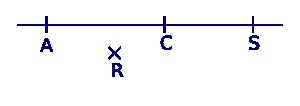
\includegraphics[width=4.3cm]{droiteARCS} \end{center} \vspace{-1em}
      \begin{ChoixQCM}{4}
      \item $R \in [AC]$
      \item $C \in [AC]$
      \item $A \in [CS]$
      \item $S \notin [AC]$
      \end{ChoixQCM}
\begin{corrige}
     \reponseQCM{bd} 
   \end{corrige}
    \end{exercice}
 
    
    \begin{exercice}
     Sur la figure ci-contre : \vspace{-2em}\begin{center}
\includegraphics[width=2.5cm]{trianglesABCDE}\end{center}\vspace{-1em}
      \begin{ChoixQCM}{4}
      \item les droites $(ED)$ et $(BC)$ sont parallèles
      \item le point $B$ appartient à la perpendiculaire à $(AC)$ passant par $D$
      \item la droite perpendiculaire à $(AB)$ passant par $D$ coupe $(AB)$ en $E$
      \item le point $A$ appartient à la  perpendiculaire à $(BC)$ passant par $E$
      \end{ChoixQCM}
\begin{corrige}
     \reponseQCM{bc}
   \end{corrige}
    \end{exercice}


    \begin{exercice}
     Dans quel(s) cas, l'équerre est‑elle bien placée pour tracer la perpendiculaire à la droite $d$ passant par le point $A$ ?
      \begin{ChoixQCM}{4}
      \item 

\begin{tikzpicture}[scale=0.55,rotate=20,every node/.style={scale=1.2}]




\draw [thick](0,0) node[above]{($d$)}--(6,0);
\draw (4,3) node[left]{A};
\draw (4,3) node[rotate=20]{$\bullet$};

%%%%%%%%%%%%%%%%%%%%%%%%
%%%%%%%%%%%%%%%%%%%%%%%%
%Définition des paramètres de l'équerre
%et de son positionnement
%%%%%%%%%%%%%%%%%%%%%%%%
%%%%%%%%%%%%%%%%%%%%%%%%

\def \xorigine {4.52}; %abscisse de l'origine de l'équerre posée avec un xshift
\def \yorigine {0}; %ordonnée de l'origine de l'équerre posée avec un yshift
\def \rotation {0}; %angle de rotation de l'équerre
\def \longueur {4}; %longueur de l'équerre
\def \largeur {2}; %largeur de l'équerre
\def \epaisseur {\longueur * 0.1}; %épaisseur de la partie «colorée» de l'équerre

%%%%%%%%%%%%%%%%%%%%%%%%
%%%%%%%%%%%%%%%%%%%%%%%%
%Tracé de l'équerre
%%%%%%%%%%%%%%%%%%%%%%%%
%%%%%%%%%%%%%%%%%%%%%%%%

\begin{scope}[scale=1,xshift=\xorigine cm,yshift=\yorigine cm,rotate=\rotation]

%contour extérieur de l'équerre
\coordinate (A) at (0,0) ; %«origine» de l'équerre
\coordinate (B) at (-\largeur,0) ;
\coordinate (C) at (0,\longueur) ;
\draw [gray](A)--(B)--(C)--cycle;


%contour intérieur de l'équerre
\coordinate (D) at (-\epaisseur,\epaisseur) ;
\coordinate (E) at ($\largeur*(-1,0)+{\largeur * \epaisseur / \longueur}*(1,0)+\epaisseur*(1,0)+\epaisseur*(0,1)$);
\coordinate (F) at ($\epaisseur*(-1,0)+\longueur*(0,1)-{2*\longueur * \epaisseur / \largeur}*(0,1)$);
\draw [gray](D)--(E)--(F)--cycle;

%partie colorée de l'équerre
\fill [color=blue!70!gray,opacity=.4,even odd rule] (A)--(B)--(C)--cycle (D)--(E)--(F)--cycle;%l'option even odd rule permet de faire le remplissage entre les 2 zones définies

\end{scope}





\end{tikzpicture}



      \item 

\begin{tikzpicture}[scale=0.55,rotate=20,every node/.style={scale=1.2}]




\draw [thick](0,0) node[above]{($d$)}--(6,0);
\draw (4.32,1.8) node[left]{A};
\draw (4.32,1.8) node{$\bullet$};

%%%%%%%%%%%%%%%%%%%%%%%%
%%%%%%%%%%%%%%%%%%%%%%%%
%Définition des paramètres de l'équerre
%et de son positionnement
%%%%%%%%%%%%%%%%%%%%%%%%
%%%%%%%%%%%%%%%%%%%%%%%%

\def \xorigine {4.32}; %abscisse de l'origine de l'équerre posée avec un xshift
\def \yorigine {1.8}; %ordonnée de l'origine de l'équerre posée avec un yshift
\def \rotation {116.8}; %angle de rotation de l'équerre
\def \longueur {4}; %longueur de l'équerre
\def \largeur {2}; %largeur de l'équerre
\def \epaisseur {\longueur * 0.1}; %épaisseur de la partie «colorée» de l'équerre

%%%%%%%%%%%%%%%%%%%%%%%%
%%%%%%%%%%%%%%%%%%%%%%%%
%Tracé de l'équerre
%%%%%%%%%%%%%%%%%%%%%%%%
%%%%%%%%%%%%%%%%%%%%%%%%

\begin{scope}[scale=1,xshift=\xorigine cm,yshift=\yorigine cm,rotate=\rotation]

%contour extérieur de l'équerre
\coordinate (A) at (0,0) ; %«origine» de l'équerre
\coordinate (B) at (-\largeur,0) ;
\coordinate (C) at (0,\longueur) ;
\draw [gray](A)--(B)--(C)--cycle;


%contour intérieur de l'équerre
\coordinate (D) at (-\epaisseur,\epaisseur) ;
\coordinate (E) at ($\largeur*(-1,0)+{\largeur * \epaisseur / \longueur}*(1,0)+\epaisseur*(1,0)+\epaisseur*(0,1)$);
\coordinate (F) at ($\epaisseur*(-1,0)+\longueur*(0,1)-{2*\longueur * \epaisseur / \largeur}*(0,1)$);
\draw [gray](D)--(E)--(F)--cycle;

%partie colorée de l'équerre
\fill [color=blue!70!gray,opacity=.4,even odd rule] (A)--(B)--(C)--cycle (D)--(E)--(F)--cycle;%l'option even odd rule permet de faire le remplissage entre les 2 zones définies

\end{scope}





\end{tikzpicture}



      \item 

\begin{tikzpicture}[scale=0.55,rotate=20,every node/.style={scale=1.2}]




\draw [thick](0,0) node[above]{($d$)}--(6,0);
\draw (4,3) node[right]{A};
\draw (4,3) node[rotate=20]{$\bullet$};

%%%%%%%%%%%%%%%%%%%%%%%%
%%%%%%%%%%%%%%%%%%%%%%%%
%Définition des paramètres de l'équerre
%et de son positionnement
%%%%%%%%%%%%%%%%%%%%%%%%
%%%%%%%%%%%%%%%%%%%%%%%%

\def \xorigine {3.95}; %abscisse de l'origine de l'équerre posée avec un xshift
\def \yorigine {0}; %ordonnée de l'origine de l'équerre posée avec un yshift
\def \rotation {0}; %angle de rotation de l'équerre
\def \longueur {4}; %longueur de l'équerre
\def \largeur {2}; %largeur de l'équerre
\def \epaisseur {\longueur * 0.1}; %épaisseur de la partie «colorée» de l'équerre

%%%%%%%%%%%%%%%%%%%%%%%%
%%%%%%%%%%%%%%%%%%%%%%%%
%Tracé de l'équerre
%%%%%%%%%%%%%%%%%%%%%%%%
%%%%%%%%%%%%%%%%%%%%%%%%

\begin{scope}[scale=1,xshift=\xorigine cm,yshift=\yorigine cm,rotate=\rotation]

%contour extérieur de l'équerre
\coordinate (A) at (0,0) ; %«origine» de l'équerre
\coordinate (B) at (-\largeur,0) ;
\coordinate (C) at (0,\longueur) ;
\draw [gray](A)--(B)--(C)--cycle;


%contour intérieur de l'équerre
\coordinate (D) at (-\epaisseur,\epaisseur) ;
\coordinate (E) at ($\largeur*(-1,0)+{\largeur * \epaisseur / \longueur}*(1,0)+\epaisseur*(1,0)+\epaisseur*(0,1)$);
\coordinate (F) at ($\epaisseur*(-1,0)+\longueur*(0,1)-{2*\longueur * \epaisseur / \largeur}*(0,1)$);
\draw [gray](D)--(E)--(F)--cycle;

%partie colorée de l'équerre
\fill [color=blue!70!gray,opacity=.4,even odd rule] (A)--(B)--(C)--cycle (D)--(E)--(F)--cycle;%l'option even odd rule permet de faire le remplissage entre les 2 zones définies

\end{scope}





\end{tikzpicture}



      \item 

\begin{tikzpicture}[scale=0.55,rotate=20,every node/.style={scale=1.2}]




\draw [thick](0,0) node[above]{($d$)}--(6,0);
\draw (4.32,2.8) node[left]{A};
\draw (4.32,2.8) node{$\bullet$};

%%%%%%%%%%%%%%%%%%%%%%%%
%%%%%%%%%%%%%%%%%%%%%%%%
%Définition des paramètres de l'équerre
%et de son positionnement
%%%%%%%%%%%%%%%%%%%%%%%%
%%%%%%%%%%%%%%%%%%%%%%%%

\def \xorigine {4.3}; %abscisse de l'origine de l'équerre posée avec un xshift
\def \yorigine {0}; %ordonnée de l'origine de l'équerre posée avec un yshift
\def \rotation {90}; %angle de rotation de l'équerre
\def \longueur {4}; %longueur de l'équerre
\def \largeur {2}; %largeur de l'équerre
\def \epaisseur {\longueur * 0.1}; %épaisseur de la partie «colorée» de l'équerre

%%%%%%%%%%%%%%%%%%%%%%%%
%%%%%%%%%%%%%%%%%%%%%%%%
%Tracé de l'équerre
%%%%%%%%%%%%%%%%%%%%%%%%
%%%%%%%%%%%%%%%%%%%%%%%%

\begin{scope}[scale=1,xshift=\xorigine cm,yshift=\yorigine cm,rotate=\rotation]

%contour extérieur de l'équerre
\coordinate (A) at (0,0) ; %«origine» de l'équerre
\coordinate (B) at (\largeur,0) ;
\coordinate (C) at (0,\longueur) ;
\draw [gray](A)--(B)--(C)--cycle;


%contour intérieur de l'équerre
\coordinate (D) at (\epaisseur,\epaisseur) ;
\coordinate (E) at ($\largeur*(1,0)-{\largeur * \epaisseur / \longueur}*(1,0)-\epaisseur*(1,0)+\epaisseur*(0,1)$);
\coordinate (F) at ($\epaisseur*(1,0)+\longueur*(0,1)-{2*\longueur * \epaisseur / \largeur}*(0,1)$);
\draw [gray](D)--(E)--(F)--cycle;

%partie colorée de l'équerre
\fill [color=blue!70!gray,opacity=.4,even odd rule] (A)--(B)--(C)--cycle (D)--(E)--(F)--cycle;%l'option even odd rule permet de faire le remplissage entre les 2 zones définies

\end{scope}





\end{tikzpicture}



      \end{ChoixQCM}
\begin{corrige}
     \reponseQCM{a}
   \end{corrige}
    \end{exercice}

   \end{GroupeQCM}  
 \end{QCM}  
 
 
 \begin{QCM}
  \begin{GroupeQCM}
    \begin{exercice}
     Soit $d_1$, $d_2$ et $d_3$ trois droites. Si $d_1 \perp d_2$ et $d_3 \perp d_2$ alors \ldots
      \begin{ChoixQCM}{4}
      \item $d_1$ et $d_3$ sont sécantes
      \item $d_2 \parallel d_3$
      \item $d_1 \perp d_3$
      \item $d_1 \parallel d_3$
      \end{ChoixQCM}
\begin{corrige}
     \reponseQCM{d}
   \end{corrige}
    \end{exercice}
    
    
  \begin{exercice}
     Sur la figure ci-contre : \vspace{-2em}\begin{center}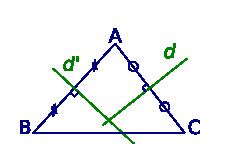
\includegraphics[width=2.9cm]{triangleABCdd}\end{center}\vspace{-1em}
      \begin{ChoixQCM}{4}
      \item $d$ est la médiatrice de $[BC]$
      \item $d$ est la médiatrice de $[AC]$
      \item $d'$ est la médiatrice de $[AB]$
      \item $d'$ est la médiatrice de $[AC]$
      \end{ChoixQCM}
\begin{corrige}
     \reponseQCM{bc}
   \end{corrige}
    \end{exercice}

     \begin{exercice}
     Si $Z$ appartient à la médiatrice de $[ST]$ alors \ldots
      \begin{ChoixQCM}{4}
      \item $ST = ZT$
      \item $ZS = ZT$
      \item $ZS = TS$
      \item $TZ = SZ$
      \end{ChoixQCM}
\begin{corrige}
     \reponseQCM{bd}
   \end{corrige}
    \end{exercice}
    

     \begin{exercice}
     Le point $A$ est le sommet des angles... \vspace{-2em}\begin{center}
\includegraphics[width=2.6cm]{sommetA}\end{center}\vspace{-1em}
      \begin{ChoixQCM}{4}
      \item $\widehat{ABC}$
      \item $\widehat{BAC}$
      \item $\widehat{DAC}$
      \item $\widehat{BDA}$
      \end{ChoixQCM}
\begin{corrige}
     \reponseQCM{bc}
   \end{corrige}
    \end{exercice}
    
    
     \begin{exercice}
     Un angle mesurant $92^\circ$ est \ldots
      \begin{ChoixQCM}{4}
      \item aigu
      \item obtus
      \item plat
      \item droit
      \end{ChoixQCM}
\begin{corrige}
     \reponseQCM{b}
   \end{corrige}
    \end{exercice}
    
    
     \begin{exercice}
     Sur la figure ci-contre : \vspace{-2em}\begin{center}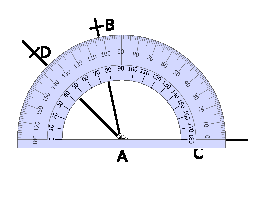
\includegraphics[width=3.8cm]{rapporteurQCM}\end{center}\vspace{-1em}
      \begin{ChoixQCM}{4}
      \item $\widehat{BAC} = 118^\circ$
      \item $\widehat{CAD} = 145^\circ$
      \item $\widehat{CAB} = 102^\circ$
      \item $\widehat{BAD} = 33^\circ$
      \end{ChoixQCM}
\begin{corrige}
     \reponseQCM{cd}
   \end{corrige}
    \end{exercice}
    
    
    \begin{exercice}
     Sur quelle(s) figure(s) la demi-droite orange est-elle la bissectrice de l'angle $\widehat{LIN}$ ?
      \begin{ChoixQCM}{4}
      \item 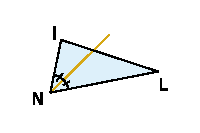
\includegraphics[width=2.2cm]{ddroite-orange1}
      \item 
\includegraphics[width=2.2cm]{ddroite-orange2}
      \item 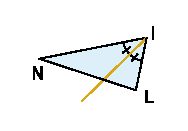
\includegraphics[width=2.2cm]{ddroite-orange3}
      \item 
\includegraphics[width=2.2cm]{ddroite-orange4}
      \end{ChoixQCM}
\begin{corrige}
     \reponseQCM{c}
   \end{corrige}
    \end{exercice}
\end{GroupeQCM}
\end{QCM}

  
